\section{Cours 5}\label{cours-5}

\subsection{Service}\label{service}

Un système d'exploitation fournit des services aux utilisateurs (aussi
distant), aux développeurs et programmes qui s'exécutent.

\subsubsection{Interface}\label{interface}

\begin{itemize}
\tightlist
\item
  Interface utilisateur: GUI ou terminal
\item
  Interface de traitement par lot: comme Inginious, on a un ensemble de
  tâches qui s'exécutent groupe par groupe. (punch card)
\end{itemize}

On retrouve la dernière interface sur les HPC et autres types de super
computer.

\paragraph{Sous linux}\label{sous-linux}

On a un système pour le batch (traitement par lot).

\begin{itemize}
\tightlist
\item
  \texttt{at}: lance une commande à un moment spécifique.
\item
  \texttt{crontab}: gérer des tâches récurrentes.
\end{itemize}

\subsubsection{Services aux concepteurs
d'applications}\label{services-aux-concepteurs-dapplications}

On facilite le déploiement d'applications sur d'autres systèmes que
celui de la machine du dev via:

\begin{itemize}
\tightlist
\item
  \textbf{Linker}: Assemble différents fichiers \emph{objets} en un
  \emph{exécutable unique}

  \begin{itemize}
  \tightlist
  \item
    \texttt{ld} sur Linux
  \item
    \texttt{-static} avec \texttt{gcc} pour avoir l'ensemble des
    libraires
  \end{itemize}
\item
  \textbf{Loader}: au démarrage d'un programme.

  \begin{itemize}
  \tightlist
  \item
    \texttt{ld.so} libraire et support du kernel Linux

    \begin{enumerate}
    \def\labelenumi{\arabic{enumi}.}
    \tightlist
    \item
      Initialise l'espace mémoire
    \item
      Pré-charge les segments text, data, environment
    \item
      Localiser et charger les libraires dynamiques
    \end{enumerate}
  \end{itemize}
\end{itemize}

Il peut aussi gérer les erreurs. ex: \emph{memory dump} pour avoir
l'état de la mémoire avant le crash. Ce \emph{memory dump} peut être
déclenché si on fait une division par 0 ou accès non autorisé à certains
segments de la mémoire.

On peut aussi facilement débugger via \texttt{gdb} et ses breakpoints.
Les breakpoints sont en réalité des \emph{trap} qui fait une
interruption logicielle !

\subsubsection{Services aux
applications}\label{services-aux-applications}

Le SE gère les entrées sorties mais il y a quelques règles:

\begin{itemize}
\tightlist
\item
  Une app \textbf{ne peut pas} envoyer d'instructions aux gestionnaires
  de périphériques
\item
  \textbf{Ne peut pas} traiter les interruptions
\item
  Hétérogénéité des périphériques eux-mêmes
\item
  SE fournit une abstraction unique pour une \emph{classe} de
  périphérique
\end{itemize}

Un des buts du SE est de faire \textbf{correspondre} des abstractions
\emph{haut niveau} et des opérations \emph{bas niveau}. On a des drivers
qui permettent de contrôler le matériel.

Un SE va partager les ressources. Il va faire:

\begin{itemize}
\tightlist
\item
  Maximisation de l'utilisation
\item
  Équité d'accès
\item
  Isolation
\end{itemize}

Il fournit aussi d'autres services spécifiques:

\begin{itemize}
\tightlist
\item
  Allocations des ressources:

  \begin{itemize}
  \tightlist
  \item
    Exclusive ou non (typique des ports)
  \item
    Contrôle générique ou spécifique
  \item
    Protection et contrôle d'accès
  \end{itemize}
\end{itemize}

\subsubsection{Accès aux services du
SE}\label{accuxe8s-aux-services-du-se}

\begin{itemize}
\tightlist
\item
  Utilisation d'utilitaire systèmes
\item
  Appel direct des fonctions du noyau
\item
  Librairie Standard
\end{itemize}

On a une API par le noyau pour les \emph{appels système}:

\begin{itemize}
\tightlist
\item
  A un numéro précis
\item
  Point d'entrée unique pour accéder aux fonctions du noyau
\end{itemize}

\paragraph{Fonctionnement}\label{fonctionnement}

\begin{enumerate}
\def\labelenumi{\arabic{enumi}.}
\tightlist
\item
  Placer les arguments dans la pile
\item
  Sauvegarde l'adresse de retour sur la pile
\item
  Modifier \texttt{\%eip} pour que la prochaine instruction à exécuter
  soit notre fonction
\item
  Fonction prend ses arguments
\item
  Sauvegarde son résultat à un endroit (\texttt{\%eax} par convention en
  IA32)
\item
  Fonction récupère l'adresse de retour sur la pile et modifie
  \texttt{\%eip} pour retourner à la fonction appelante.
\end{enumerate}

\begin{figure}
\centering
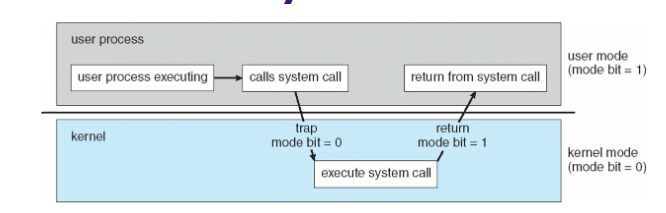
\includegraphics{image-12.png}
\caption{Alt text}
\end{figure}

On change de mode d'exécution. On change d'espace mémoire !

\paragraph{Réalisation concrète}\label{ruxe9alisation-concruxe8te}

Problème 1: placer des arguments qui seront accessibles par le noyau. On
va le mettre soit dans:

\begin{itemize}
\tightlist
\item
  Un espace mémoire fixe dédié (data)
\item
  Sur la pile
\item
  Registres (\texttt{\%ebx} pour premier argument puis \texttt{\%ecx})
\end{itemize}

Problème 2: adresse de retour

\begin{itemize}
\tightlist
\item
  Pointeur de programme sauvegardé sur la pile.
\item
  Restauré au retour
\end{itemize}

Problème 3: appel effectif

\begin{itemize}
\tightlist
\item
  Passer en mode protégé
\item
  Instructions spéciales (IA32 \texttt{int\ 0x80} crée une interruption)
  ou simplement \texttt{syscall}.
\item
  Point d'entrée du kernel est connu par le processeur.
\end{itemize}

\begin{figure}
\centering
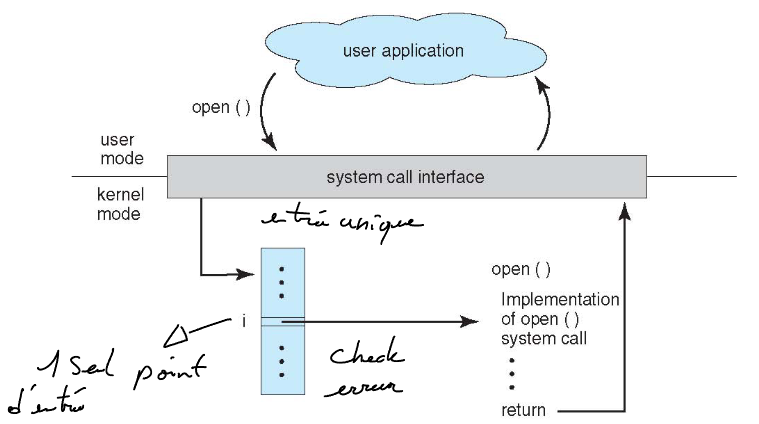
\includegraphics{image-13.png}
\caption{Alt text}
\end{figure}

Problème 4: récupération du code de retour

\begin{enumerate}
\def\labelenumi{\arabic{enumi}.}
\tightlist
\item
  Opération autorisée et paramètre corrects:

  \begin{itemize}
  \tightlist
  \item
    Résultat mis dans le registre \texttt{\%eax}
  \item
    Instruction de retour au mode utilisateur, dépile l'adresse de
    retour et positionne le compteur de programme
  \end{itemize}
\item
  Erreur ou opération non autorisée

  \begin{itemize}
  \tightlist
  \item
    Positionne la variable d'environnement \texttt{errno}
  \item
    Retourne aux processus parent (ex: shell)
  \end{itemize}
\end{enumerate}

\paragraph{Appels systèmes}\label{appels-systuxe8mes}

\begin{itemize}
\tightlist
\item
  Librairie standard: s'exécute dans le même espace mémoire que le
  programme utilisateur. \texttt{printf(3)} va forcément utiliser
  \texttt{write(2)} ou autres opérations bas niveau.
\item
  \texttt{strace(1)} permet de tracer les appels systèmes utilisés par
  un processus
\end{itemize}

\begin{figure}
\centering
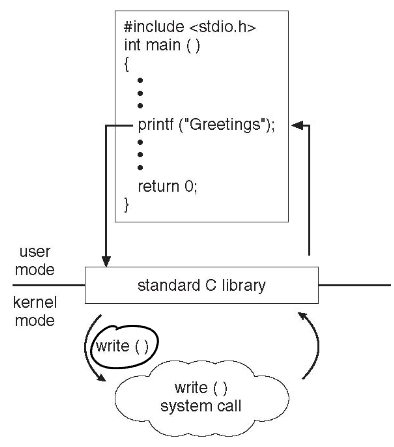
\includegraphics{image-14.png}
\caption{Alt text}
\end{figure}

\paragraph{Hello world}\label{hello-world}

\begin{Shaded}
\begin{Highlighting}[]
\PreprocessorTok{\#include }\ImportTok{\textless{}stdio.h\textgreater{}}
\PreprocessorTok{\#include }\ImportTok{\textless{}stdlib.h\textgreater{}}

\DataTypeTok{int}\NormalTok{ main}\OperatorTok{(}\DataTypeTok{int}\NormalTok{ argc}\OperatorTok{,} \DataTypeTok{char} \OperatorTok{*}\NormalTok{argv}\OperatorTok{[])\{}
\NormalTok{   printf}\OperatorTok{(}\StringTok{"Hello, world! }\SpecialCharTok{\%d\textbackslash{}n}\StringTok{"}\OperatorTok{,}\KeywordTok{sizeof}\OperatorTok{(}\DataTypeTok{int}\OperatorTok{));}
   \ControlFlowTok{return}\NormalTok{ EXIT\_SUCCESS}\OperatorTok{;}
\OperatorTok{\}}
\end{Highlighting}
\end{Shaded}

Traduction:

\begin{Shaded}
\begin{Highlighting}[]
\NormalTok{$ strace ./helloworld\_s}
\NormalTok{execve("./helloworld\_s", ["./helloworld\_s"], [/* 21 vars */]) = 0}
\NormalTok{uname(\{sys="Linux", node="precise32", ...\}) = 0}
\NormalTok{brk(0)                                  = 0x9e8b000}
\NormalTok{brk(0x9e8bd40)                          = 0x9e8bd40}
\NormalTok{set\_thread\_area(\{entry\_number:{-}1 {-}\textgreater{} 6, base\_addr:0x9e8b840, limit:1048575, seg\_32bit:1, }
\NormalTok{contents:0, read\_exec\_only:0, limit\_in\_pages:1, seg\_not\_present:0, useable:1\}) = 0}
\NormalTok{brk(0x9eacd40)                          = 0x9eacd40}
\NormalTok{brk(0x9ead000)                          = 0x9ead000}
\NormalTok{fstat64(1, \{st\_mode=S\_IFCHR|0620, st\_rdev=makedev(136, 0), ...\}) = 0}
\NormalTok{mmap2(NULL, 4096, PROT\_READ|PROT\_WRITE, MAP\_PRIVATE|MAP\_ANONYMOUS, {-}1, 0) = 0xb778a000}
\NormalTok{write(1, "Hello, world! 4\textbackslash{}n", 16Hello, world! 4}
\NormalTok{)       = 16}
\NormalTok{exit\_group(0)                           = ?}
\end{Highlighting}
\end{Shaded}

\subsection{Architecture des systèmes
d'exploitation}\label{architecture-des-systuxe8mes-dexploitation}

\begin{figure}
\centering
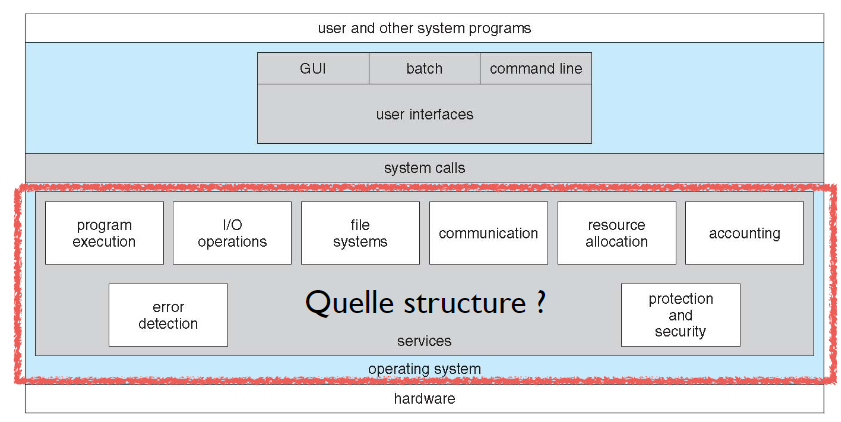
\includegraphics{image-15.png}
\caption{Alt text}
\end{figure}

\subsubsection{Objectifs et contraintes de mise en oeuvre d'un
SE}\label{objectifs-et-contraintes-de-mise-en-oeuvre-dun-se}

\begin{itemize}
\tightlist
\item
  Pas de modèle unique et parfait
\item
  Contraintes et objectifs:

  \begin{itemize}
  \tightlist
  \item
    Contraintes du matériel
  \item
    Performance et coût d'implémentation
  \item
    Consommation de ressources
  \item
    Facilité d'évolution et d'adaptation
  \item
    Facilité de maintenance et d'atteinte de fiabilité
  \end{itemize}
\end{itemize}

\subsubsection{MS-DOS}\label{ms-dos}

SE des systèmes \emph{IBM-PC} pas basé sur UNIX, c'est Microsoft.

Objectifs:

\begin{itemize}
\tightlist
\item
  Mono-utilisateur et mono-application (Pas de temps partagé)
\item
  Visant des processeurs \textbf{ne supportant pas} les modes
  utilisateur/protégé (Pas d'isolation)
\item
  Contrainte forte sur l'utilisation de la mémoire (coutait extrêmement
  cher à l'époque)
\end{itemize}

Système avec une vision \textbf{monolithique} pour éviter de consommer
trop de mémoire.

\begin{figure}
\centering
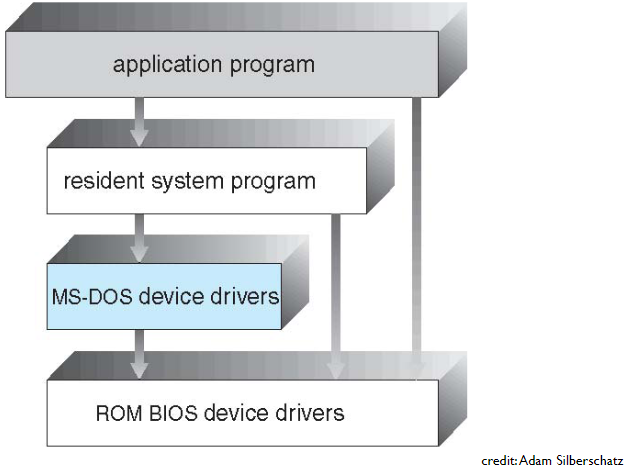
\includegraphics{image-16.png}
\caption{Alt text}
\end{figure}

\begin{figure}
\centering
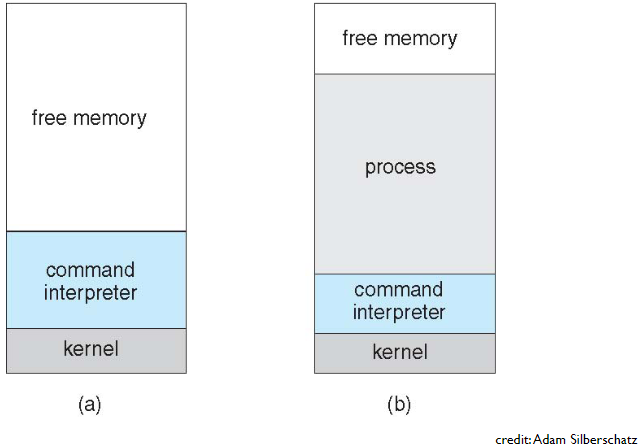
\includegraphics{image-17.png}
\caption{Alt text}
\end{figure}

\subsubsection{UNIX}\label{unix}

\paragraph{Monolithe}\label{monolithe}

Plus vieux que \hyperref[ms-dos]{MS-DOS} mais pensé pour des ordinateurs
à plus grande capacité.

\begin{itemize}
\tightlist
\item
  Multi utilisateur et temps partagé
\item
  Processeur supportant les deux modes
\item
  Séparation claire entre \emph{noyau} et \emph{programmes utilisateurs}
\end{itemize}

Organisation originelle: \emph{monolithe}:

\begin{itemize}
\tightlist
\item
  1 seul programme sur 1 seule couche, met en oeuvre tous les appels
  systèmes
\item
  Difficile à étendre, adapter, débugger
\end{itemize}

\begin{figure}
\centering
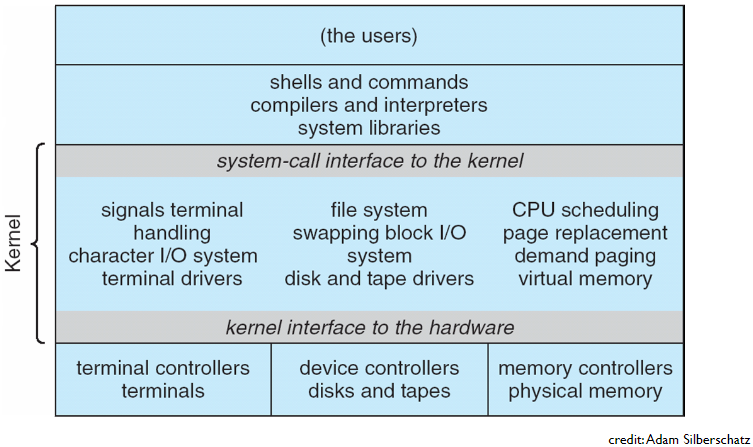
\includegraphics{image-18.png}
\caption{Alt text}
\end{figure}

\paragraph{Couches}\label{couches}

On va rajouter de la structure pour pallier aux soucis lié à
\hyperref[monolithe]{unix monolithique}

Les couches:

\begin{enumerate}
\def\labelenumi{\arabic{enumi}.}
\tightlist
\item
  Matériel
\item
  Drivers de périphériques
\item
  Abstractions des plus en plus haut niveau, jusqu'aux appels systèmes
\item
  Interface utilisateur
\end{enumerate}

\begin{figure}
\centering
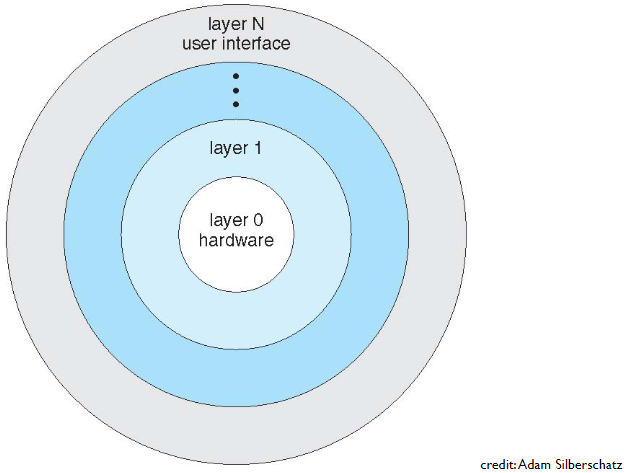
\includegraphics{image-19.png}
\caption{Alt text}
\end{figure}

Il y a des avantages et inconvénients !

Avantages:

\begin{itemize}
\tightlist
\item
  Isolations des fonctionnalités
\item
  Facilité de portage
\end{itemize}

Inconvénients:

\begin{itemize}
\tightlist
\item
  Surcoût à l'exécution des appels système
\item
  Difficile de décider d'une structure purement hiérarchique.

  \begin{itemize}
  \tightlist
  \item
    Il y a une interdépendance entre les fonctions du SE
  \end{itemize}
\end{itemize}

\paragraph{Structure en Modules}\label{structure-en-modules}

\begin{figure}
\centering
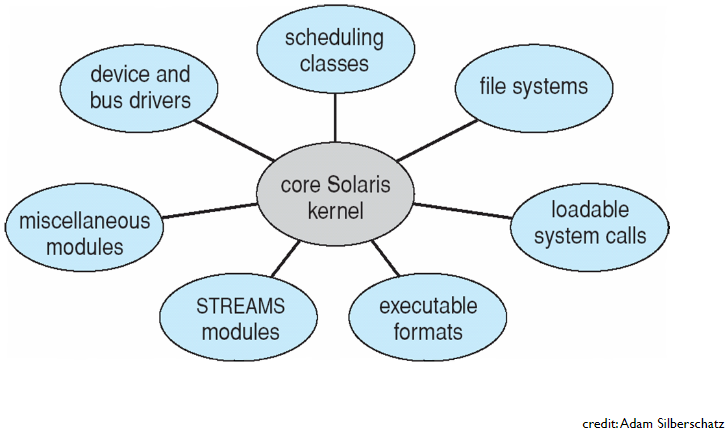
\includegraphics{image-20.png}
\caption{Alt text}
\end{figure}

Utilisé le plus souvent: Linux, Solaris, Windows

On a un coeur qui est un monolithe ou qui a peu de couche.

\begin{itemize}
\tightlist
\item
  Gestion bas niveau de la mémoire
\item
  Gestion des processus
\end{itemize}

Le reste est sous forme de modules:

\begin{itemize}
\tightlist
\item
  Charges et décharges de l'espace mémoire du noyau \emph{dynamiquement}
\item
  Seulement lorsque nécessaire

  \begin{itemize}
  \tightlist
  \item
    Ex: quand on met une clé usb. Va charger \texttt{exFAT} si clé
    venant de Windows
  \end{itemize}
\end{itemize}

Avantages:

\begin{itemize}
\tightlist
\item
  Spécialisation d'une SE pour un environnement donné:

  \begin{itemize}
  \tightlist
  \item
    Versatilité de Linux
  \end{itemize}
\item
  Interactions possibles entre les modules en conservant la séparation
  de code et de mémoire.

  \begin{itemize}
  \tightlist
  \item
    Analogie possible avec programmation orientée objet
  \end{itemize}
\end{itemize}

Inconvénients:

\begin{itemize}
\tightlist
\item
  Surcoût (négligeable sur les systèmes modernes)
\item
  Intégration de modules écrits par des tiers dans l'espace mémoire du
  noyau

  \begin{itemize}
  \tightlist
  \item
    potentiels bugs et fautes
  \end{itemize}
\end{itemize}

Gestions des modules sous Linux (seulement si \texttt{root}):

\begin{itemize}
\tightlist
\item
  \texttt{lsmod}: liste les modules présents
\item
  \texttt{modprobe}: ajoute/supprime un module
\item
  \texttt{modinfo}: information sur un module
\end{itemize}

\subsubsection{Macro- et Micro-noyaux}\label{macro--et-micro-noyaux}

\paragraph{Macro-noyaux}\label{macro-noyaux}

Tous les modes précédents placent l'intégralité des fonctions du SE dans
le noyau.

\begin{itemize}
\tightlist
\item
  Toutes s'exécutent en mode protégé
\item
  Accès complet à la mémoire et aux instructions sensibles
\item
  Crash du module = \textbf{crash du système}
\end{itemize}

Le kernel est en pérille, corruption des données, faille pour les
hackers.

\paragraph{Micro-noyaux}\label{micro-noyaux}

Séparation entre un noyau minimaliste

\begin{itemize}
\tightlist
\item
  Gestion basique de la mémoire
\item
  Gestion des processus légers (threads)
\item
  Gestion de la communication entre processus (IPC)
\end{itemize}

Le reste est mis en oeuvre par des processus en mode utilisateur (même
les drivers)

Réduit les bugs de modules et évitent les crash complets tout en gardant
les propriétés d'isolation.

\begin{figure}
\centering
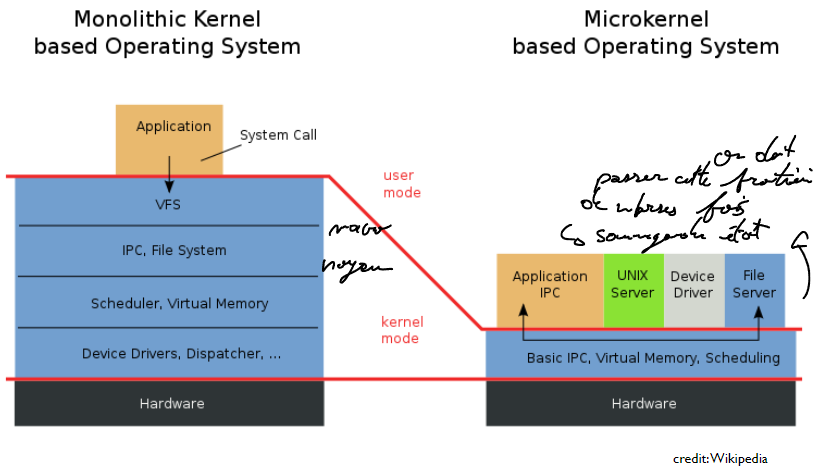
\includegraphics{image-21.png}
\caption{Alt text}
\end{figure}

Inconvénients:

\begin{itemize}
\tightlist
\item
  En macro: appel de module dans un même espace mémoire donc très
  rapide. En micro: il faut faire des appels systèmes

  \begin{itemize}
  \tightlist
  \item
    Copie de l'argument de l'appelant vers le noyau
  \item
    Copie dans l'espace mémoire de l'appelé
  \item
    Changement de contexte (sauvegarde du contexte et
    restauration\ldots)
  \item
    \ldots{} et rebelote dans l'autre sens pour la valeur de retour
  \end{itemize}
\end{itemize}

Donc on a longtemps abandonnés les micro-noyaux (abandon dans Windows
NT) MAIS:

\begin{itemize}
\tightlist
\item
  Progrès sensibles dans la mise en oeuvre des appels systèmes
\item
  Passage de message en mode zero-copy
\item
  Mac OS et iOS proche d'un micro-noyau
\end{itemize}

\subsubsection{Fiabilité des SE}\label{fiabilituxe9-des-se}

Souvent beaucoup de temps nécessaires pour corriger des fautes.
Énormément de fautes dans les drivers et compliqués à débugger et
trouver parfois.

\paragraph{Certification formelle}\label{certification-formelle}

Pour les systèmes embarqués critiques on réalise des
\textbf{spécification formelle}. On modélise \emph{mathématiquement}
qu'un système est fiable. C'est le cas pour seL4. Mais seulement
possible si le code est petit.

\subsubsection{Démarrage du SE}\label{duxe9marrage-du-se}

Démarrage et reset de la machine: interruption de mise à zéro du
processeur. 2 phases:

\begin{enumerate}
\def\labelenumi{\arabic{enumi}.}
\tightlist
\item
  Programme de démarrage (bootstrap) stocké dans une ROM. Charge ainsi
  le bootloader
\item
  Bootloader lit les systèmes de fichiers pour charger l'image du noyau
  en mémoire (\texttt{/boot/vmlinuz-3.12.0-32-generic}) en gros le GRUB.
\end{enumerate}
